\section{Theorie}

Licht ist eine elektromagnetische Welle. Wenn eine Lichtwelle demnach in Materie
eindringt hat sie durch die Wechselwirkung mit Elektronen eine geringere
Ausbreitungsgeschwindigkeit als in Vakuum. Das führt dazu, dass ein Lichtstrahl,
der schräg in ein Material eindringt an der Grenzfläche gebrochen wird.
Dieser Vorgang kann durch das \enquote{Huygenssche Prinzip} beschrieben werden.
Es besagt, dass jeder Punkt einer Wellenfront als Zentrum einer neuen kugelförmigen
Elementarwelle angesehen werden kann und diese Elementarwellen überlagern dann sich zu einer
neuen Wellenfront.
Die Brechung wird durch den Brechungsindex $n$ beschrieben, welcher durch das
Verhältnis der beiden Lichtgeschwindigkeiten definiert ist

\begin{equation}
  n = \frac{c}{v} = \frac{v_1}{v_2}.
  \label{eq:1}
\end{equation}

Mithilfe von Winkelbeziehungen kann aus dieser Gleichung das
\enquote{Snelliussche Brechungsgesetz} hergeleitet werden

\begin{equation}
  n = \frac{\sin(\alpha)}{\sin(\beta)}
  \label{eq:2}
\end{equation}

Dabei ist $\alpha$ der Einfallswinkel eines Lichtstrahls gegen die Normale
der Grenzfläche und $\beta$ der Winkel gegen die Normale nach der Brechung.

Des Weiteren ist der Brechungsindex abhängig von der Frequenz $\omega$ des Lichtes,
da Licht eine elektromagnetische Welle ist. Das wird als Dispersion bezeichnet. Um
eine Gleichung für die Dispersion herzuleiten wird von der Maxwellschen Theorie
für elektromagnetische Wellen ausgegangen.

Die Kraft die durch das elektrische Feld auf die Ladungen $q_h$ in der Materie wirkt ergibt
sich zu

\begin{equation*}
  \vec{F_e} = q_h \vec{E_0} \exp(i \omega t).
\end{equation*}

Außerdem wirkt auf diese Ladungen $q_h$ aufgrund der Auslenkung aus ihrer Ruhelage
eine rücktreibende Kraft

\begin{equation*}
  \vec{F_{r,h}} = a_h \vec{x_h}
\end{equation*}

wobei $\vec{x_h}$ die Auslenkung ist. Zudem wirkt noch eine Reibungskraft, welche die
periodische Bewegung dämpft

\begin{equation*}
  \vec{F_{d,h}} = f_h \frac{d \vec{x_h}}{dt}.
\end{equation*}

Mit diesen Kräften lässt sich nun eine Differentialgleichung aufstellen. Nun lässt sich
die Auslenkung $\vec{x_h}$ noch durch die Polarisation $\vec{P_h}$ ausdrücken

\begin{equation*}
  \vec{P} = \sum_h \vec{P_h} = \sum_h = N_h q_h \vec{x_h}.
\end{equation*}

Dabei sind $N_h$ die Ladungsträger pro Volumeneinheit. Damit ergibt sich die
Differentialgleichung

\begin{equation*}
  \frac{d^2\vec{P_h}}{dt^2} + \frac{f_h}{m_h} \frac{d\vec{P_h}}{dt} + \frac{a_h}{m_h} \vec{P_h}
  = \frac{N_h q_h^2}{m_h} \vec{E_0} \exp(i \omega t).
\end{equation*}

Für die Polarisation gilt der Zusammenhang

\begin{equation*}
  \vec{P} = (\epsilon - 1) \epsilon_0 \vec{E}
\end{equation*}

und für die Dielektrizitätskonstante $\epsilon$ gilt

\begin{equation*}
  \epsilon = n^2.
\end{equation*}

Damit wird nun aus der Lösung dieser Differentialgleichung eine Gleichung für die
Dispersion hergeleitet

\begin{equation*}
  n^2(\lambda) = 1 + \sum_h \frac{N_h q_h^2}{4 \pi^2 c^2 \epsilon_0 m_h} \frac{\lambda^2 \lambda_h^2}{\lambda - \lambda_h}.
\end{equation*}

Für die Annahme, dass das Material nur eine Absorptionsstelle hat gilt $\lambda_h = \lambda_1$ und
in der Gleichung ist $\lambda$ die Wellenlänge ausserhalb des Materials.
Nun kann diese Gleichung Taylorentwickelt werden. Unter der Annahme $\lambda >> \lambda_1$
ergibt sich

\begin{equation}
  n^2(\lambda) = A_0 + \frac{A_2}{\lambda^2} + \frac{A_4}{\lambda^4} + \dotsb
  \label{eq:3}
\end{equation}

und unter der Annahme $\lambda << \lambda_1$ ergibt sich

\begin{equation}
  n^2(\lambda) = 1 - A´_2 \lambda^2 - A´_4 \lambda^4 - \dotsb
  \label{eq:4}
\end{equation}

Diese Gleichungen sind nur geeignet Dispersion von Gläsern im sichtbaren
Spektralbereich zu beschreiben. Außerhalb dieses Bereiches kommt es zu Resonanzeffekten
und somit zu hohen einer Absorption des Festkörpers.
Die typischen Kurvenverläufe dieser Kurven sind in Abbildung \ref{abb:1} dargestellt.

\begin{figure}[H]
  \centering
  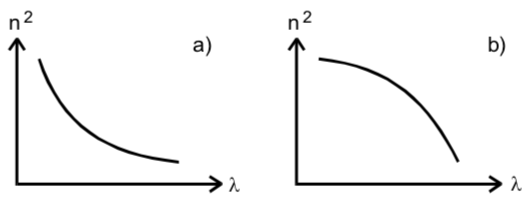
\includegraphics[width=\textwidth]{content/Dispersion.png}
  \caption{Typische Gestalt der Dispersionskurven. In a) nach \ref{eq:3} und in b) nach \ref{eq:4}. \cite{1}}
  \label{abb:1}
\end{figure}

Normale Dispersion bedeutet, dass der Brechungsindex bei zunehmender Wellenlänge abnimmt
und abnormale Dispersion, dass der Brechungsindex bei zunehmender Wellenlänge zunimmt.
